\documentclass{beamer}
\setbeamercovered{transparent}


\usetheme{CambridgeUS}
\setbeamercolor{normal text}{bg=gray!20}
\setbeamertemplate{blocks}[default]
\setbeamercolor{block title}{fg=white,bg=red!60!black}
\setbeamercolor{block body}{fg=black,bg=gray!15}

\usepackage[latin1]{inputenc}
\usepackage{amsmath}
\usepackage{amsthm}
\usepackage{amsfonts}
\usepackage{graphicx}
\usepackage{amssymb}
\usepackage{epsfig}
\usepackage{fancyhdr}
\usepackage{psfrag}
\usepackage{pstricks}
\usepackage{colortbl}
\usepackage{longtable}
\usepackage[scriptsize,tight]{subfigure}
\usepackage{multimedia}
\usepackage{color}
\usepackage{fancybox}
\usepackage{comment}
\usepackage{ragged2e}


\usefonttheme[onlymath]{serif}


\setbeamertemplate{navigation symbols}{}  


\author[Teor�a de Circuitos]{Teor�a de Circuitos}
\title[Tema 3]{\scshape Tema 3}
\subtitle{Fuentes reales y circuitos equivalentes}

\date[]{}
\institute[ETSI]{Departamento de Ingenier�a El�ctrica \\ Escuela T�cnica Superior de Ingenier�a\\ Universidad de Sevilla}


\AtBeginSection[]{
\begin{frame}
\frametitle{�ndice}
\tableofcontents[currentsection]
\end{frame}
}


\begin{document}



\begin{frame}
\titlepage
\end{frame}

\begin{frame}
\frametitle{�ndice}
%\tableofcontents[pausesections]
\tableofcontents
\end{frame}



\section[]{Fuente real de tensi�n continua}

\begin{frame}
\frametitle{Fuente real de tensi�n continua}

\begin{block}{Algunas observaciones}

\begin{enumerate}
  \justifying
  \item Toda fuente real tiene una potencia m�xima que puede suministrar.
  \item La tensi�n en bornes de una fuente real de tensi�n depende del circuito al que se conecte.
  \item Las fuentes reales sufren un calentamiento durante su uso.
\end{enumerate}
\end{block}

\begin{block}{Modelo lineal de una fuente real de tensi�n}
\vspace*{-0.2cm}
\begin{figure}[hbt]
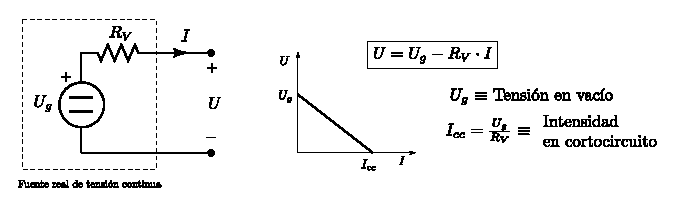
\epsfig{file=./figuras_tema_3/f_tension_real.eps,height=3cm}
\end{figure}
\end{block}
\end{frame}



\section[]{Fuente real de corriente continua}

\begin{frame}
\frametitle{Fuente real de corriente continua}
\begin{block}{Algunas observaciones}

\begin{enumerate}
	\justifying
  \item Toda fuente real tiene una potencia m�xima que puede suministrar.
  \item La intensidad en bornes de una fuente real de corriente depende del circuito al que se conecte.
  \item Las fuentes reales sufren un calentamiento durante su uso.
\end{enumerate}
\end{block}

\begin{block}{Modelo lineal y caracter�stica $U$-$I$}
\vspace*{-0.2cm}
\begin{figure}[hbt]

\epsfig{file=./figuras_tema_3/f_intensidad_real.eps,height=3cm}
\end{figure}
\end{block}

\end{frame}

\section[]{Equivalencia entre fuentes reales}

\begin{frame}
\frametitle{Equivalencia entre fuentes reales}
\justifying
Para toda fuente real de tensi�n existe una fuente real de corriente equivalente, y viceversa.
\begin{figure}[hbt]
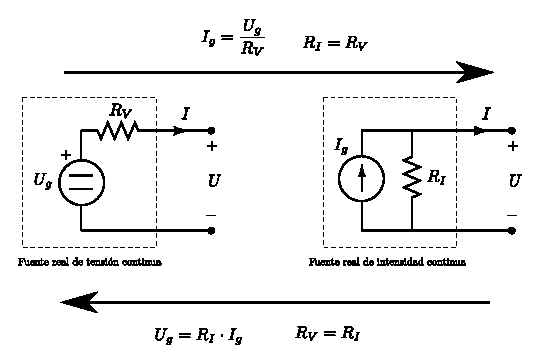
\epsfig{file=./figuras_tema_3/equivalencia_fuentes.eps,height=6.5cm}
\end{figure}

\end{frame}

\section[]{Asociaci�n de fuentes reales}

\begin{frame}
\frametitle{Asociaci�n de fuentes reales conectadas en serie}
\justifying
Varias fuentes reales de tensi�n en serie pueden agruparse en una �nica fuente equivalente. En el caso de fuentes reales de corriente, primero habr�a que obtener sus respectivas fuentes reales de tensi�n equivalentes.
\begin{figure}[hbt]

\epsfig{file=./figuras_tema_3/f_tension_serie.eps,height=6cm}
\label{f_tension_serie}
\end{figure}

\end{frame}

\begin{frame}
\frametitle{Asociaci�n de fuentes reales conectadas en paralelo}
\justifying
Varias fuentes reales de corriente en paralelo pueden agruparse en una �nica fuente equivalente. En el caso de fuentes reales de tensi�n, primero habr�a que obtener sus respectivas fuentes reales de corriente equivalentes.
\begin{figure}[hbt]

\epsfig{file=./figuras_tema_3/f_int_paralelo.eps,height=6cm}
\label{f_int_paralelo}
\end{figure}

\end{frame}




\section[]{Circuitos equivalente Th�venin y Norton}

\begin{frame}\frametitle{Circuito equivalente Th�venin}

\justifying
Todo circuito compuesto exclusivamente por fuentes y resistencias equivale a una fuente real de tensi�n (equivalente Th�venin).

\begin{columns}
\begin{column}{8cm}
\begin{figure}[hbt]
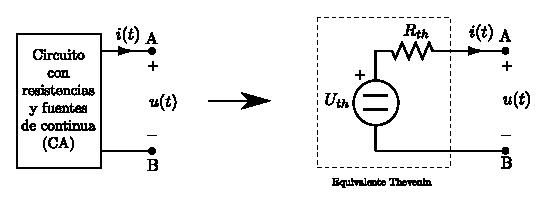
\epsfig{file=./figuras_tema_3/thevenin.eps,height=2.5cm}
\end{figure}
\end{column}
\begin{column}{3cm}
$$\boxed{U_{th}=\left.u_{ca}\right|_{{AB}}}$$
$$\boxed{R_{th}=\left.R_{eq}\right|_{{AB}}}$$
\end{column}
\end{columns}

\vspace{0.5cm}

El valor de la tensi�n de la fuente ideal es el que presenta el circuito original a intensidad nula (circuito abierto), mientras que la resistencia equivalente es la que presenta el circuito original anuladas las fuentes (circuito pasivo).

\end{frame}

\begin{frame}\frametitle{Circuito equivalente Norton}
	
\justifying
Todo circuito compuesto exclusivamente por fuentes y resistencias equivale a una fuente real de intensidad (equivalente Norton).
	
\begin{columns}
\begin{column}{8cm}
\begin{figure}[hbt]
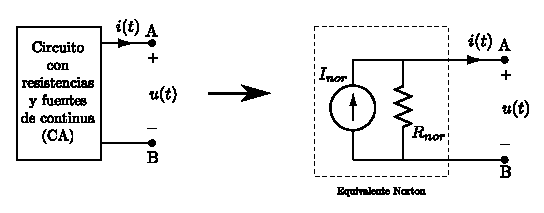
\epsfig{file=./figuras_tema_3/norton.eps,height=2.5cm}
\end{figure}
\end{column}
\begin{column}{3cm}
$$\boxed{I_{nor}=\left.i_{cc}\right|_{{AB}}}$$
$$\boxed{R_{nor}=\left.R_{eq}\right|_{{AB}}}$$
\end{column}
\end{columns}

\vspace{0.5cm}

El valor de la corriente de la fuente ideal es el que presenta el circuito original a tensi�n nula (cortocircuito), mientras que la resistencia equivalente es la que presenta el circuito original anuladas las fuentes (circuito pasivo).

\end{frame}

\begin{frame}\frametitle{Circuitos equivalente Th�venin y Norton}
\begin{columns}
  \begin{column}{4cm}

\begin{block}{Obtenci�n de $u_{ca}$ e $i_{cc}$}

\begin{small}
Se obtienen resolviendo los circuitos siguientes:
\end{small}

  \begin{figure}[hbt]
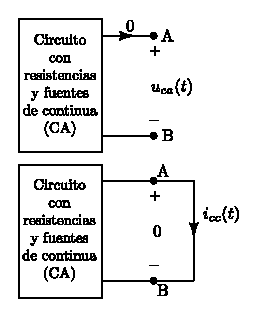
\epsfig{file=./figuras_tema_3/calculo_equiv_1.eps,height=4.3cm}
\end{figure}

\begin{small}
	\textbf{CA}: circuito activo.
\end{small}

\end{block}
\end{column}
\begin{column}{7.5cm}

\begin{block}{Obtenci�n de $R_{eq}$}

\begin{small}
   \textbf{1� forma}: A partir de $u_{ca}$ y $i_{cc}$:
    
    \begin{equation*}
    R_{eq}=\frac{u_{ca}}{i_{cc}}, \ \  \text{salvo indeterminaci�n:}\ 0/0
\end{equation*}


   \textbf{2� forma}: Conectando al circuito pasivo una fuente de prueba externa. Esto es:
 
   \begin{columns}
   \begin{column}{2cm}
   \begin{equation*}
   R_{eq}=\cfrac{U_g}{I_g}
   \end{equation*}
         \end{column}
   \begin{column}{5cm}
      \begin{figure}[hbt]
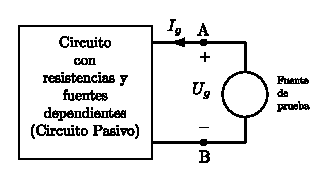
\epsfig{file=./figuras_tema_3/calculo_equiv_2.eps,height=2.5cm}
\end{figure}
   \end{column}
  \end{columns}
  \vspace{0.1cm}
    \textbf{3� forma}: Asociaci�n de resistencias del circuito pasivo.
    \textit{No aplicable si hay fuentes dependientes}.
\end{small}

\end{block}
\end{column}
\end{columns}

\end{frame}



\begin{frame}
\begin{exampleblock}{Ejercicio 3.1}
	\justifying
En el circuito en corriente continua de la figura, se pide obtener el equivalente de Th�venin entre los terminales a y b.

\begin{figure}[hbt]
\centering
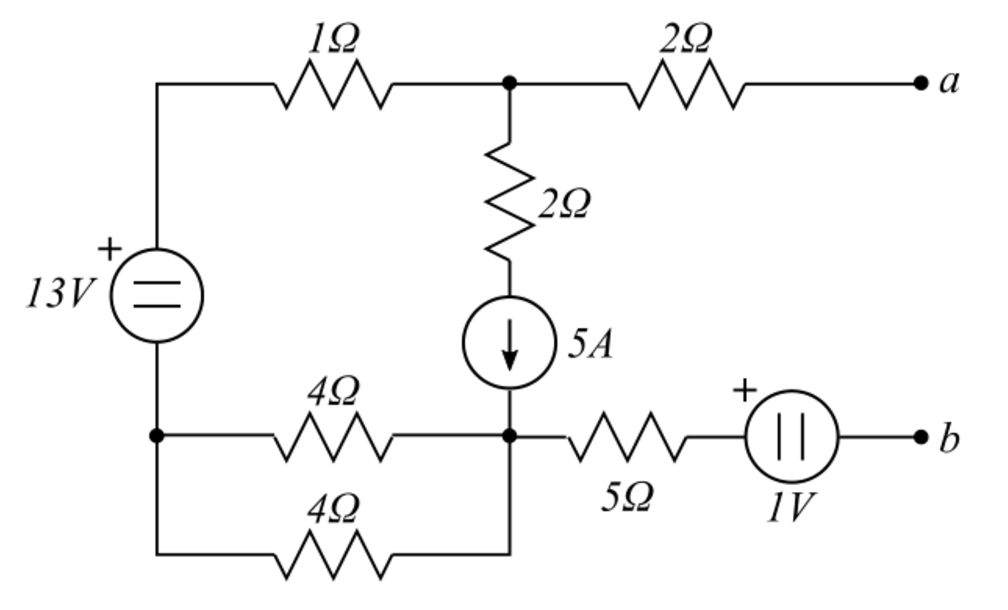
\epsfig{file=./figuras_tema_3/Ej_The.eps,height=3.5cm}
\end{figure}

\textbf{Soluci�n}: $U_{th}=-1$ V, $R_{th}=10 \, \mathrm{\Omega}$

\end{exampleblock}
\end{frame}



\section{M�xima transferencia de potencia}

\begin{frame}
\frametitle{M�xima potencia de una fuente real de tensi�n}
\vspace{-0.5cm}
\begin{columns}
\begin{column}{5cm}
\begin{figure}[hbt]
\fboxsep 1pt
\fcolorbox{blue}{white}{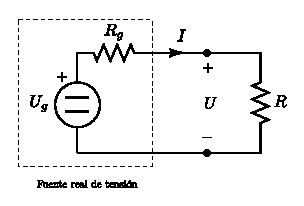
\epsfig{file=./figuras_tema_3/max_pot_DC.eps,height=3cm}}
\end{figure}
\end{column}
\begin{column}{6cm}
$P=U I=R I^2=\cfrac{R}{(R+R_g)^2}\cdot U^2_g$
$$P_{max} \ \ \Longrightarrow \ \ \frac{dP}{dR}=0 \ \ \Rightarrow  \ \ \boxed{R=R_g}$$
\end{column}
\end{columns}
%\vspace{0.5cm}
%$$P_{max} \ \ \Longrightarrow \ \ \frac{dP}{dR}=0 \ \ \Rightarrow  \ \ \boxed{R=R_g}$$

%\vspace{-0.2cm}
\begin{columns}[t]
\begin{column}{6cm}
\begin{itemize}
\item Potencia m�xima:
\begin{small}
  \begin{equation*}
    P_{max}=\frac{U^2_g}{4\cdot R_g}
  \end{equation*}
  \end{small}
  \vspace{-0.5cm}
 \item Rendimiento:
 \begin{small}
  \begin{equation*}
    \eta=\frac{U I}{U_g  I}=\frac{R}{R+R_g}
  \end{equation*}
  Si $R=R_g \ \ \Rightarrow \ \ \left.\eta \right|_{P_{max}}=0.5$
    \end{small}
  \end{itemize}
  \vspace{-0.8cm}
   \end{column}

\begin{column}{6cm}
  \vspace{-0.5cm}
 \begin{figure}[hbt]
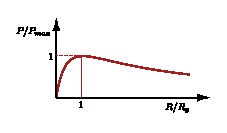
\epsfig{file=./figuras_tema_3/graf_pot_max.eps,height=2.5cm}
\end{figure}

\vspace{-1.2cm}
     \begin{figure}[hbt]
     \hspace*{0.5cm}
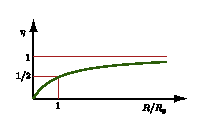
\epsfig{file=./figuras_tema_3/graf_rend.eps,height=2.5cm}
\end{figure}
\end{column}
\end{columns}

\end{frame}




\begin{frame}
\frametitle{M�xima potencia de una fuente real de intensidad}
\vspace{-0.5cm}
\begin{columns}
\begin{column}{5cm}
\begin{figure}[hbt]
\fboxsep 1pt
\fcolorbox{blue}{white}{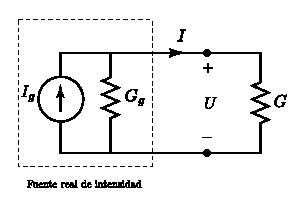
\epsfig{file=./figuras_tema_3/max_pot_DC_2.eps,height=3cm}}
\end{figure}
\end{column}
\begin{column}{6cm}
$P=U I=G U^2=\cfrac{G}{(G+G_g)^2}\cdot I^2_g$
$$P_{max} \ \ \Longrightarrow \ \ \frac{dP}{dR}=0 \ \ \Rightarrow  \ \ \boxed{G=G_g}$$
\end{column}
\end{columns}
%\vspace{0.5cm}
%$$P_{max} \ \ \Longrightarrow \ \ \frac{dP}{dR}=0 \ \ \Rightarrow  \ \ \boxed{R=R_g}$$

%\vspace{-0.2cm}
\begin{columns}[t]
\begin{column}{6cm}
\begin{itemize}
\item Potencia m�xima:
\begin{small}
  \begin{equation*}
    P_{max}=\frac{I^2_g}{4\cdot G_g}
  \end{equation*}
  \end{small}
  \vspace{-0.5cm}
 \item Rendimiento:
 \begin{small}
  \begin{equation*}
    \eta=\frac{U I}{U  I_g}=\frac{G}{G+G_g}
  \end{equation*}
  Si $G=G_g \ \ \Rightarrow \ \ \left.\eta \right|_{P_{max}}=0.5$
    \end{small}
  \end{itemize}
  \vspace{-0.8cm}
   \end{column}

\begin{column}{6cm}
  \vspace{-0.5cm}
 \begin{figure}[hbt]
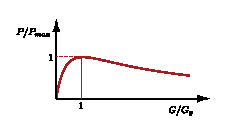
\epsfig{file=./figuras_tema_3/graf_pot_max_2.eps,height=2.5cm}
\end{figure}

\vspace{-1.2cm}
     \begin{figure}[hbt]
     \hspace*{0.5cm}
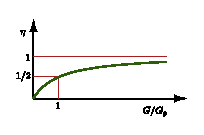
\epsfig{file=./figuras_tema_3/graf_rend_2.eps,height=2.5cm}
\end{figure}
\end{column}
\end{columns}

\end{frame}

\begin{frame}
	\begin{exampleblock}{Ejercicio 3.2}
		\justifying
		Determinar el valor de la resistencia R para que la fuente real de intensidad trabaje con un rendimiento del 80 \%. Datos: $R_g = 4 \, \mathrm{k\Omega}$
		.
		\begin{figure}[hbt]
			\centering
			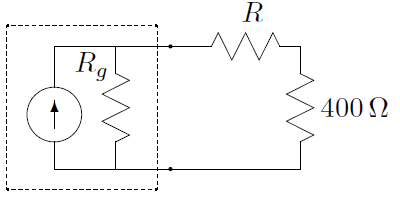
\includegraphics[height=3.5cm]{./figuras_tema_3/Ej_3_2.PNG}
		\end{figure}
		\textbf{Soluci�n}: $R=600 \, \mathrm{\Omega}$
	\end{exampleblock}
\end{frame}


\end{document}


